\documentclass[10pt,aspectratio=169]{beamer}

%% ── Theme ────────────────────────────────────────────────────────────────────
\usetheme{Madrid}
\usecolortheme{default}

\definecolor{darkblue}{RGB}{0,51,102}
\definecolor{lightblue}{RGB}{220,235,250}
\definecolor{accentred}{RGB}{180,30,30}
\definecolor{accentgreen}{RGB}{0,110,60}
\definecolor{midgray}{RGB}{100,100,100}

\setbeamercolor{structure}{fg=darkblue}
\setbeamercolor{title}{fg=white,bg=darkblue}
\setbeamercolor{frametitle}{fg=darkblue,bg=lightblue}
\setbeamercolor{block title}{fg=white,bg=darkblue}
\setbeamercolor{block body}{bg=lightblue}

\setbeamerfont{frametitle}{size=\small,series=\bfseries}
\setbeamertemplate{navigation symbols}{}
\setbeamertemplate{footline}{%
  \hfill\insertframenumber/\inserttotalframenumber\hspace{0.5cm}\vspace{0.3cm}%
}

%% ── Packages ─────────────────────────────────────────────────────────────────
\usepackage{amsmath,amssymb}
\usepackage{graphicx}
\usepackage{tikz}
\usetikzlibrary{arrows.meta,positioning,calc}
\usepackage{booktabs}
\usepackage{appendixnumberbeamer}
\usepackage{pgfpages}
%% Uncomment the next line to show notes during practice:
%\setbeameroption{show notes on second screen=right}

%% ── Metadata ─────────────────────────────────────────────────────────────────
\title[Stayers' Innovation in Pharma M\&A]{\textbf{After the Acquisition}}
\subtitle{Post-Merger Innovation Among Stayers in Pharma M\&A}
\author{Tim K\"{u}hleis \\[0.5em]
        \small Regulation, Markets and Environment Research Seminar\\[-0.1em]
        \small Paris School of Economics}
\date{April 2026}

\begin{document}

\begin{frame}
  \titlepage
\end{frame}
\note{Thank the organizers and introduce yourself briefly. This is a master's thesis presentation on what happens to inventors inside pharmaceutical firms after they are acquired --- specifically, to those who stay.}

%% ════════════════════════════════════════════════════════════════════════════
%% Slide 1 — Motivation and research question
%% ════════════════════════════════════════════════════════════════════════════
\begin{frame}{Pharma Mergers Raise Innovation Concerns That Remain Unanswered for Retained Inventors}

\begin{columns}[T]

  \column{0.48\textwidth}
  \textbf{Why this matters}
  \begin{itemize}\small
    \item High concentration, frequent M\&A, and exceptionally high R\&D intensity make pharma the central industry for studying merger-innovation links
    \item FTC 2023 \textit{Multilateral Pharmaceutical Merger Task Force}: ``What is the full range of a pharma merger's effects on innovation?''
  \end{itemize}

  \column{0.48\textwidth}
  \textbf{What the literature establishes}
  \begin{itemize}\small
    \item Patenting falls 10--30\% post-merger at the firm level (Ornaghi 2009; Haucap et al.\ 2019)
    \item Exit and departure rates spike; exiters and movers each lose ${\sim}$30\% of expected career output (Cassi \& Ornaghi 2026)
    \item \textbf{Open gap:} productivity, quality, and field trajectories of inventors who \textit{stay} remain unexplored
  \end{itemize}

\end{columns}

\vspace{0.5em}
\begin{block}{Research Question}
\small Do acquisitions reduce the patent quantity, citation-weighted quality, and technological focus of target-firm inventors who remain with the acquiring group --- and does technological overlap between acquirer and target determine which channel dominates?
\end{block}

\end{frame}

\note{Start with the policy hook. The pharmaceutical sector is interesting for two reasons: it is one of the most R\&D-intensive industries in the world, and it has been consolidating aggressively for decades. That combination has put it squarely on the radar of competition authorities.

In 2023 the FTC formally asked: what is the full range of a merger's effects on innovation? That is almost exactly the question I am trying to answer, just at a more granular level.

The literature gives us two layers of evidence. At the firm level, we know patenting falls after mergers. At the inventor level, Cassi and Ornaghi --- whose data I am using --- show that exit and departure rates spike, and that inventors who leave lose around 30 percent of their expected career output.

But there is a group nobody has looked at carefully: the inventors who stay. They are the majority --- Cassi and Ornaghi report that roughly 73 percent of target inventors remain. And yet we know almost nothing about what happens to the quality or direction of their research after the deal. That is the gap I am addressing. The key addition relative to my first presentation: I now ask not just whether disruption reduces output, but whether technological overlap determines which of two competing channels dominates.}

%% ════════════════════════════════════════════════════════════════════════════
%% Slide 2 — Two-channel framework and hypotheses
%% ════════════════════════════════════════════════════════════════════════════
\begin{frame}{Two Channels Predict Opposing Effects --- Post-Merger Frictions Dominate in Pharma}

\begin{columns}[T]

  \column{0.50\textwidth}

  {\color{accentred}\textbf{Post-merger frictions} $\rightarrow$ lower output}
  \begin{itemize}\footnotesize
    \item Integration frictions divert attention from discovery (Kapoor \& Lim 2007)
    \item Loss of status reduces motivation for central inventors (Paruchuri et al.\ 2006)
    \item Disrupted knowledge networks limit access to tacit knowledge (Ernst \& Vitt 2000)
    \item Weaker championing of early-stage projects (Hitt et al.\ 1991)
  \end{itemize}

  \vspace{0.3em}
  {\color{accentgreen}\textbf{Internalized spillovers} $\rightarrow$ higher output}
  \begin{itemize}\footnotesize
    \item Mergers internalize informational externalities across R\&D teams (Das et al.\ 2023)
    \item Hybrid target--acquirer coinvention raises citation impact (Li \& Wang 2022)
    \item Bridge-building inventors gain ${\sim}$10\% patenting boost (Sharoni 2026)
  \end{itemize}

  \vspace{0.2em}
  {\scriptsize\color{midgray}\textit{Net effect theoretically ambiguous. Frictions predicted to dominate in pharma: knowledge is tacit, integration costs are severe.}\par}

  \column{0.48\textwidth}

  \textbf{Hypotheses}
  \begin{itemize}\footnotesize
    \item[\color{accentred}\textbf{H1}] Acquisition reduces stayer patent \textit{quantity}
    \item[\color{accentred}\textbf{H2}] Acquisition reduces citation-weighted \textit{quality}
    \item[\color{accentred}\textbf{H3}] Stayers exhibit \textit{TechDrift}: shift into acquirer's fields
    \item[\color{accentgreen}\textbf{H4}] Negative H1/H2 effects attenuated when acquirer--target technological overlap is high (\textit{DealSim})
    \item[\color{accentgreen}\textbf{H5}] Stayers who coinvent with acquirer-side inventors suffer smaller losses
  \end{itemize}

  \vspace{0.3em}
  \textbf{Friction heterogeneity}
  \vspace{0.1em}
  {\footnotesize
  \begin{tabular}{@{}p{3.2cm}r@{}}
  \toprule
  Interaction & Sign \\
  \midrule
  Age $\times$ After & $+$ \\
  Exclusivity $\times$ After & $-$ \\
  Big deal $\times$ After & $-$ \\
  \bottomrule
  \end{tabular}}

\end{columns}

\end{frame}

\note{I want to flag the key change from my first presentation: I now frame the theoretical prediction as ambiguous rather than one-sided.

Two channels operate simultaneously. Post-merger frictions run through integration costs, loss of status, disrupted networks, and weaker project championing --- all reducing inventor output. Internalized spillovers run in the opposite direction: mergers remove the free-rider problem in R&D and hybrid coinvention teams can be more productive than either firm separately.

The honest IO answer, grounded in the Bourreau-Jullien-Lefouili framework, is that the net sign is ambiguous. I predict frictions dominate in pharma specifically because pharmaceutical knowledge is highly tacit and integration costs are empirically severe. H1 through H3 test this baseline prediction. H4 and H5 are the spillover-channel tests: does technological proximity (DealSim) attenuate the negative ATT, and is active coinvention the actual conduit?

Crucially, CommonIPC was in my heterogeneity table in the first presentation. I have elevated it to H4 because it is theoretically a spillover test, not a friction moderator.}

%% ════════════════════════════════════════════════════════════════════════════
%% Slide 3 — Data
%% ════════════════════════════════════════════════════════════════════════════
\begin{frame}{One Million Inventor-Year Observations Spanning 513 Acquisitions Form the Empirical Foundation}

\begin{columns}[T]

  \column{0.48\textwidth}
  \textbf{Base data --- Cassi \& Ornaghi (2026, \textit{EER})}
  \begin{itemize}\small
    \item EPO/PatStat (v.\ 2017) and Orbis/Zephyr (Bureau van Dijk)
    \item 311,358 inventors; 1,000,751 inventor $\times$ year obs., 1988--2015
    \item 513 pharma acquisitions; avg.\ 3.21 observations per inventor
    \item Upstream cleaning taken as given: disambiguation, original-applicant recovery, dynamic group construction
  \end{itemize}

  \column{0.48\textwidth}
  \textbf{Own additions}
  \begin{itemize}\small
    \item DuckDB/R pipeline: \texttt{inventor\_year}, \texttt{inventor\_ipc\_year}, \texttt{group\_ipc\_year}
    \item OECD Patent Quality Indicators (PQII) linked via application ID: originality, radicalness, claims, composite score
    \item \textit{TechDrift}$_{it}$ (H3): IPC cosine similarity to inventor's pre-merger baseline
    \item \textit{DealSim}$_c$ (H4): pre-deal cosine similarity of acquirer and target IPC portfolios
    \item \textit{Coinventor indicator} (H5): stayer files $\geq$1 post-deal joint patent with an acquirer-side inventor
  \end{itemize}

\end{columns}

\vspace{0.6em}
{\footnotesize\color{midgray}\centering
TechDrift and DealSim both use binary IPC vectors. Declining TechDrift signals field misallocation; high DealSim signals technological overlap between merging firms. See formulas on final slide.\par}

\end{frame}

\note{The base data is unchanged. Let me focus on what I have added.

TechDrift works as before: I construct a binary IPC vector for each inventor in each year and compute cosine similarity to their pre-merger baseline vector built from the five years before the deal. A score of one means same fields as before; a declining score means drift into new territory.

DealSim is the new measure for H4. I apply the same cosine similarity logic at the deal level: pre-deal IPC portfolios for the target group and the acquiring group, measured over the five years before the acquisition. This gives one number per deal capturing how technologically similar the two firms were. High DealSim means more overlapping knowledge to internalize and less organizational distance to cross.

The coinventor indicator for H5 uses the patent-inventor bridge table. An acquirer-side inventor is someone who filed patents for the acquiring group pre-deal but never for the target. A stayer is a coinventor if they share at least one post-deal patent with any acquirer-side inventor within three years of the deal. Together these three measures let me test not just whether frictions reduce output on average, but whether internalized spillovers --- through proximity and active coinvention --- offset some of that loss.}

%% ════════════════════════════════════════════════════════════════════════════
%% Slide 4 — Empirical strategy
%% ════════════════════════════════════════════════════════════════════════════
\begin{frame}{CS(2021) Tests Net Effects; DealSim and Coinventor Splits Isolate the Spillover Channel}

\begin{columns}[T]

  \column{0.50\textwidth}
  \textbf{Sample and estimator}
  \begin{itemize}\small
    \item \textit{Treated stayer:} $\geq$1 patent for target (5 pre-deal years), continues filing for acquiring group within $x \in \{3,5\}$ years; acquirer-side inventors excluded
    \item \textit{Control:} not-yet-treated --- more comparable than structurally different never-treated firms
    \item Callaway \& Sant'Anna (2021) group-time ATT, doubly robust\\
    {\footnotesize Covariates: PrePatents, Age, Tenure, Exclusivity, FirmPatentStock}
  \end{itemize}

  \vspace{0.3em}
  \textbf{Outcomes tested (H1--H3)}
  \begin{itemize}\small
    \item $Y_{it} \in \{$Patents, FracPatents, Citations, Quality$_{\text{PQII}}$, TechDrift$\}$
    \item Event study $\tau \in [-5,+5]$ validates parallel trends (Roth 2022)
    \item Aggregate ATT gives the main result for each outcome
  \end{itemize}

  \column{0.48\textwidth}

  \textbf{Spillover-channel tests (H4--H5)}

  \vspace{0.4em}
  {\small\textit{H4 --- DealSim moderation:}}
  \begin{itemize}\footnotesize
    \item Re-estimate CS by DealSim tercile (low / mid / high)
    \item Prediction: $|\text{ATT}|$ shrinks monotonically with overlap
    \item Robustness: TWFE with DealSim $\times$ After interaction
  \end{itemize}

  \vspace{0.5em}
  {\small\textit{H5 --- Coinventor split:}}
  \begin{itemize}\footnotesize
    \item Re-estimate CS for coinventing vs.\ non-coinventing stayers
    \item Prediction: non-coinventing stayers drive the negative ATT; coinventing stayers show attenuation
    \item Explains Cassi \& Ornaghi's collaborator finding mechanically
  \end{itemize}

\end{columns}

\end{frame}

\note{The core identification strategy is unchanged: Callaway and Sant'Anna with not-yet-treated controls and doubly robust estimation. I use not-yet-treated rather than never-treated because never-treated pharma firms are structurally different --- the ones nobody wanted to acquire.

For H1 through H3, I run five separate CS estimations. The event study plots validate parallel trends and give the dynamic picture. The aggregate ATT gives the summary number. The sign prediction is negative for patents, citations, quality, and TechDrift.

For H4, I split by DealSim tercile. The prediction is monotone: low-overlap deals show the largest negative ATT, high-overlap deals the smallest. I use tercile splits because continuous-moderator interaction within CS is non-standard; TWFE with DealSim-times-After serves as robustness.

For H5, I split by coinventor status. Non-coinventing stayers should drive the aggregate negative ATT; coinventing stayers should show near-zero or attenuated effects. This gives a structural interpretation for the Cassi and Ornaghi finding that collaborating stayers are barely affected by mergers.}

%% ════════════════════════════════════════════════════════════════════════════
%% Slide 5 — Equations
%% ════════════════════════════════════════════════════════════════════════════
\begin{frame}{Formal Framework: Estimating Equations and Novel Measures}

\begin{columns}[T]

  \column{0.50\textwidth}
  \textbf{CS(2021) estimating equations}

  \vspace{0.4em}
  {\small Event study (dynamic ATT):}
  \[
    Y_{ict} = \sum_{\tau=-5}^{+5}
    \lambda_\tau \cdot \mathbf{1}[t - g_c = \tau]
    + \alpha_i + \xi_{ct} + \varepsilon_{ict}
  \]
  {\footnotesize\color{midgray}Pre-treatment coefficients test parallel trends (Roth 2022).\par}

  \vspace{0.5em}
  {\small Aggregate ATT:}
  \[
    Y_{ict} = \lambda \cdot \text{After}_{ict}
    + \alpha_i + \xi_{ct} + \varepsilon_{ict}
  \]
  {\footnotesize\color{midgray}
  $\alpha_i$: inventor fixed effects \quad $\xi_{ct}$: firm $\times$ year FE\\[0.2em]
  {\color{accentred}$\lambda < 0$}: post-acquisition decline in output.\par}

  \column{0.48\textwidth}
  \textbf{Novel similarity measures}

  \vspace{0.4em}
  {\small Field misallocation (H3):}
  \[
    \text{TechDrift}_{it} =
    \frac{\mathbf{v}_{i}^{t} \cdot \mathbf{v}_{i}^{0}}
         {\|\mathbf{v}_{i}^{t}\|\,\|\mathbf{v}_{i}^{0}\|}
  \]
  {\footnotesize\color{midgray}Declining values: inventor drifts into unfamiliar fields post-merger.\par}

  \vspace{0.5em}
  {\small Technological overlap (H4):}
  \[
    \text{DealSim}_{c} =
    \frac{\mathbf{v}_{\text{target}}^{\text{pre}} \cdot \mathbf{v}_{\text{acq}}^{\text{pre}}}
         {\|\mathbf{v}_{\text{target}}^{\text{pre}}\|\,\|\mathbf{v}_{\text{acq}}^{\text{pre}}\|}
  \]
  {\footnotesize\color{midgray}High values: acquirer and target share technology fields --- internalized spillovers more active.\par}

\end{columns}

\end{frame}

\note{This slide collects the formal framework for reference.

On the left, the two CS estimating equations. The event study runs from five years before the deal to five years after. The pre-treatment coefficients are the parallel trends test: if they are flat and close to zero, the identifying assumption holds. The aggregate ATT collapses the dynamic picture to a single number. Both equations include inventor fixed effects --- absorbing time-invariant differences in inventor productivity --- and firm-times-year fixed effects, which control for any time-varying shocks at the firm level.

On the right, the two cosine similarity measures share the same IPC-vector architecture but operate at different levels of observation. TechDrift is measured at the inventor level and tracks how the inventor's technology profile changes over time relative to their own pre-merger baseline. DealSim is measured at the deal level and captures how similar the acquirer and target were before the merger. A high DealSim means the two firms were working in overlapping fields, which the spillover channel says should produce better outcomes for stayers --- more to internalize, less organizational distance to bridge.}

%% ════════════════════════════════════════════════════════════════════════════
%% Slide 6 — Contributions and policy
%% ════════════════════════════════════════════════════════════════════════════
\begin{frame}{Stayer Effects Reveal a Missing Channel of Dynamic Welfare Loss in Pharma Merger Review}

\vspace{0.3em}
\textbf{Novel contributions}

\vspace{0.3em}
\begin{columns}[T]
  \column{0.32\textwidth}
  {\small\color{accentred}\textbf{Quality and field outcomes}}\\[0.3em]
  {\footnotesize First quality-adjusted test of stayer performance using OECD PQII and TechDrift --- prior work measures raw patent counts only.}

  \column{0.32\textwidth}
  {\small\color{accentgreen}\textbf{Spillover-channel tests}}\\[0.3em]
  {\footnotesize H4 and H5 identify \textit{when} and \textit{through what conduit} internalized spillovers offset frictions, operationalizing Bourreau--Jullien--Lefouili at inventor level.}

  \column{0.32\textwidth}
  {\small\color{darkblue}\textbf{Identification}}\\[0.3em]
  {\footnotesize CS(2021) staggered DiD with doubly robust estimation, heterogeneity analysis, and Heckman selection correction at inventor level.}
\end{columns}

\vspace{0.6em}
\begin{center}
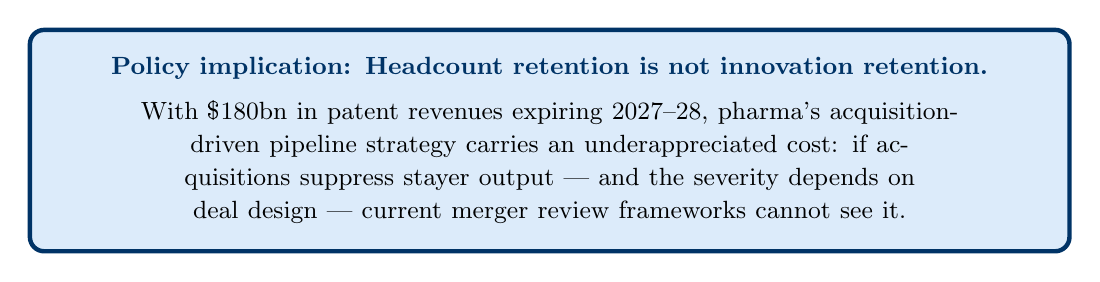
\begin{tikzpicture}
  \node[draw=darkblue, ultra thick, fill=lightblue, rounded corners=1.2ex,
        text width=12.5cm, align=center, inner sep=10pt] {
    {\small\bfseries\color{darkblue}Policy implication: Headcount retention is not innovation retention.}\\[0.4em]
    {\small With \$180bn in patent revenues expiring 2027--28, pharma's acquisition-driven pipeline strategy
    carries an underappreciated cost: if acquisitions suppress stayer output --- and the severity depends on deal design ---
    current merger review frameworks cannot see it.}
  };
\end{tikzpicture}
\end{center}

\end{frame}

\note{Let me close with why the expanded framework makes the contribution stronger.

The previous version of this paper predicted one direction of effects and tested for it. The new version frames the question as genuinely ambiguous and provides tests of both channels. That is a better science story and a more useful policy contribution, because it tells regulators not just that stayers are hurt on average, but which deal characteristics make the outcome worse or better.

H4 and H5 together operationalize the Bourreau-Jullien-Lefouili framework at the inventor level. A deal with high DealSim and active post-deal coinvention is one where the spillover channel is alive. The policy implication is different from a deal with low overlap and no coinvention, where pure frictions dominate.

On policy: the key argument is that current merger review treats the stayer problem as solved once you count who stayed. This paper says that is not enough. Even retained inventors may produce less and worse research --- and the damage depends on deal design. That is a question merger review can act on.

The patent cliff makes this urgent. Pharma companies facing 180 billion dollars in patent expirations are actively acquiring to refill pipelines. If those acquisitions suppress the innovation productivity of the very scientists being retained, the strategy is partially self-defeating --- and this evidence speaks directly to it.

Happy to take questions.}

\end{document}
